%%% template.tex
%%%
%%% This LaTeX source document can be used as the basis for your technical
%%% paper or abstract.

%%% The parameter to the ``documentclass'' command is very important.
%%% - use ``review'' for content submitted for review.
%%% - use ``preprint'' for accepted content you are making available.
%%% - use ``tog'' for technical papers accepted to the TOG journal and
%%%   for presentation at the SIGGRAPH or SIGGRAPH Asia conference.
%%% - use ``conference'' for final content accepted to a sponsored event
%%%   (hint: If you don't know, you should use ``conference.'')

\documentclass[tog]{acmsiggraph}

%%% Make the ``BibTeX'' word pretty...

\def\BibTeX{{\rm B\kern-.05em{\sc i\kern-.025em b}\kern-.08em
    T\kern-.1667em\lower.7ex\hbox{E}\kern-.125emX}}

%%% Used by the ``review'' variation; the online ID will be printed on 
%%% every page of the content.

\TOGonlineid{45678}

%%% Used by the ``preprint'' variation.

\TOGvolume{0}
\TOGnumber{0}

\title{
    Project 1: Deep-Q-Learning-for-Navigation\\
    {\large Udacity Deep Reinforcement Learning Nanodegree Program}
}

\author{
    Bob Flagg
    \thanks{
        \href{
            http://github.com/bobflagg/Deep-Q-Learning-for-Navigation}{\underline{Deep-Q-Learning-for-Navigation}}
    }
}

%\author{Rahul dfsd\thanks{e-mail:rahul.shome@cs.rutgers.edu}\\Teaching Assistant}
\pdfauthor{author1}

\keywords{Reinforcement Learning, Deep Learning}

%using a package
\usepackage{amssymb}
\usepackage{amsmath}

%Macros
%This defines the command \R which prints a Blackboard bold capital R.
\newcommand{\R}{\mathbb{R}}

%This defines the command \bb{} which prints the passed parameter in Blackboard
%bold style. It's a shorter version of the command \mathbb{}
\newcommand{\bb}[1]{\mathbb{#1}}

%Command with an optional command
\newcommand{\plusbinomial}[3][2]{(#2 + #3)^#1}

%For tables
\usepackage[utf8]{inputenc}
\usepackage[table]{xcolor}

\setlength{\arrayrulewidth}{1mm}
\setlength{\tabcolsep}{18pt}
\renewcommand{\arraystretch}{2.5}

\usepackage[section]{placeins}

\begin{document}

%%% This is the ``teaser'' command, which puts an figure, centered, below 
%%% the title and author information, and above the body of the content.

 \teaser{
   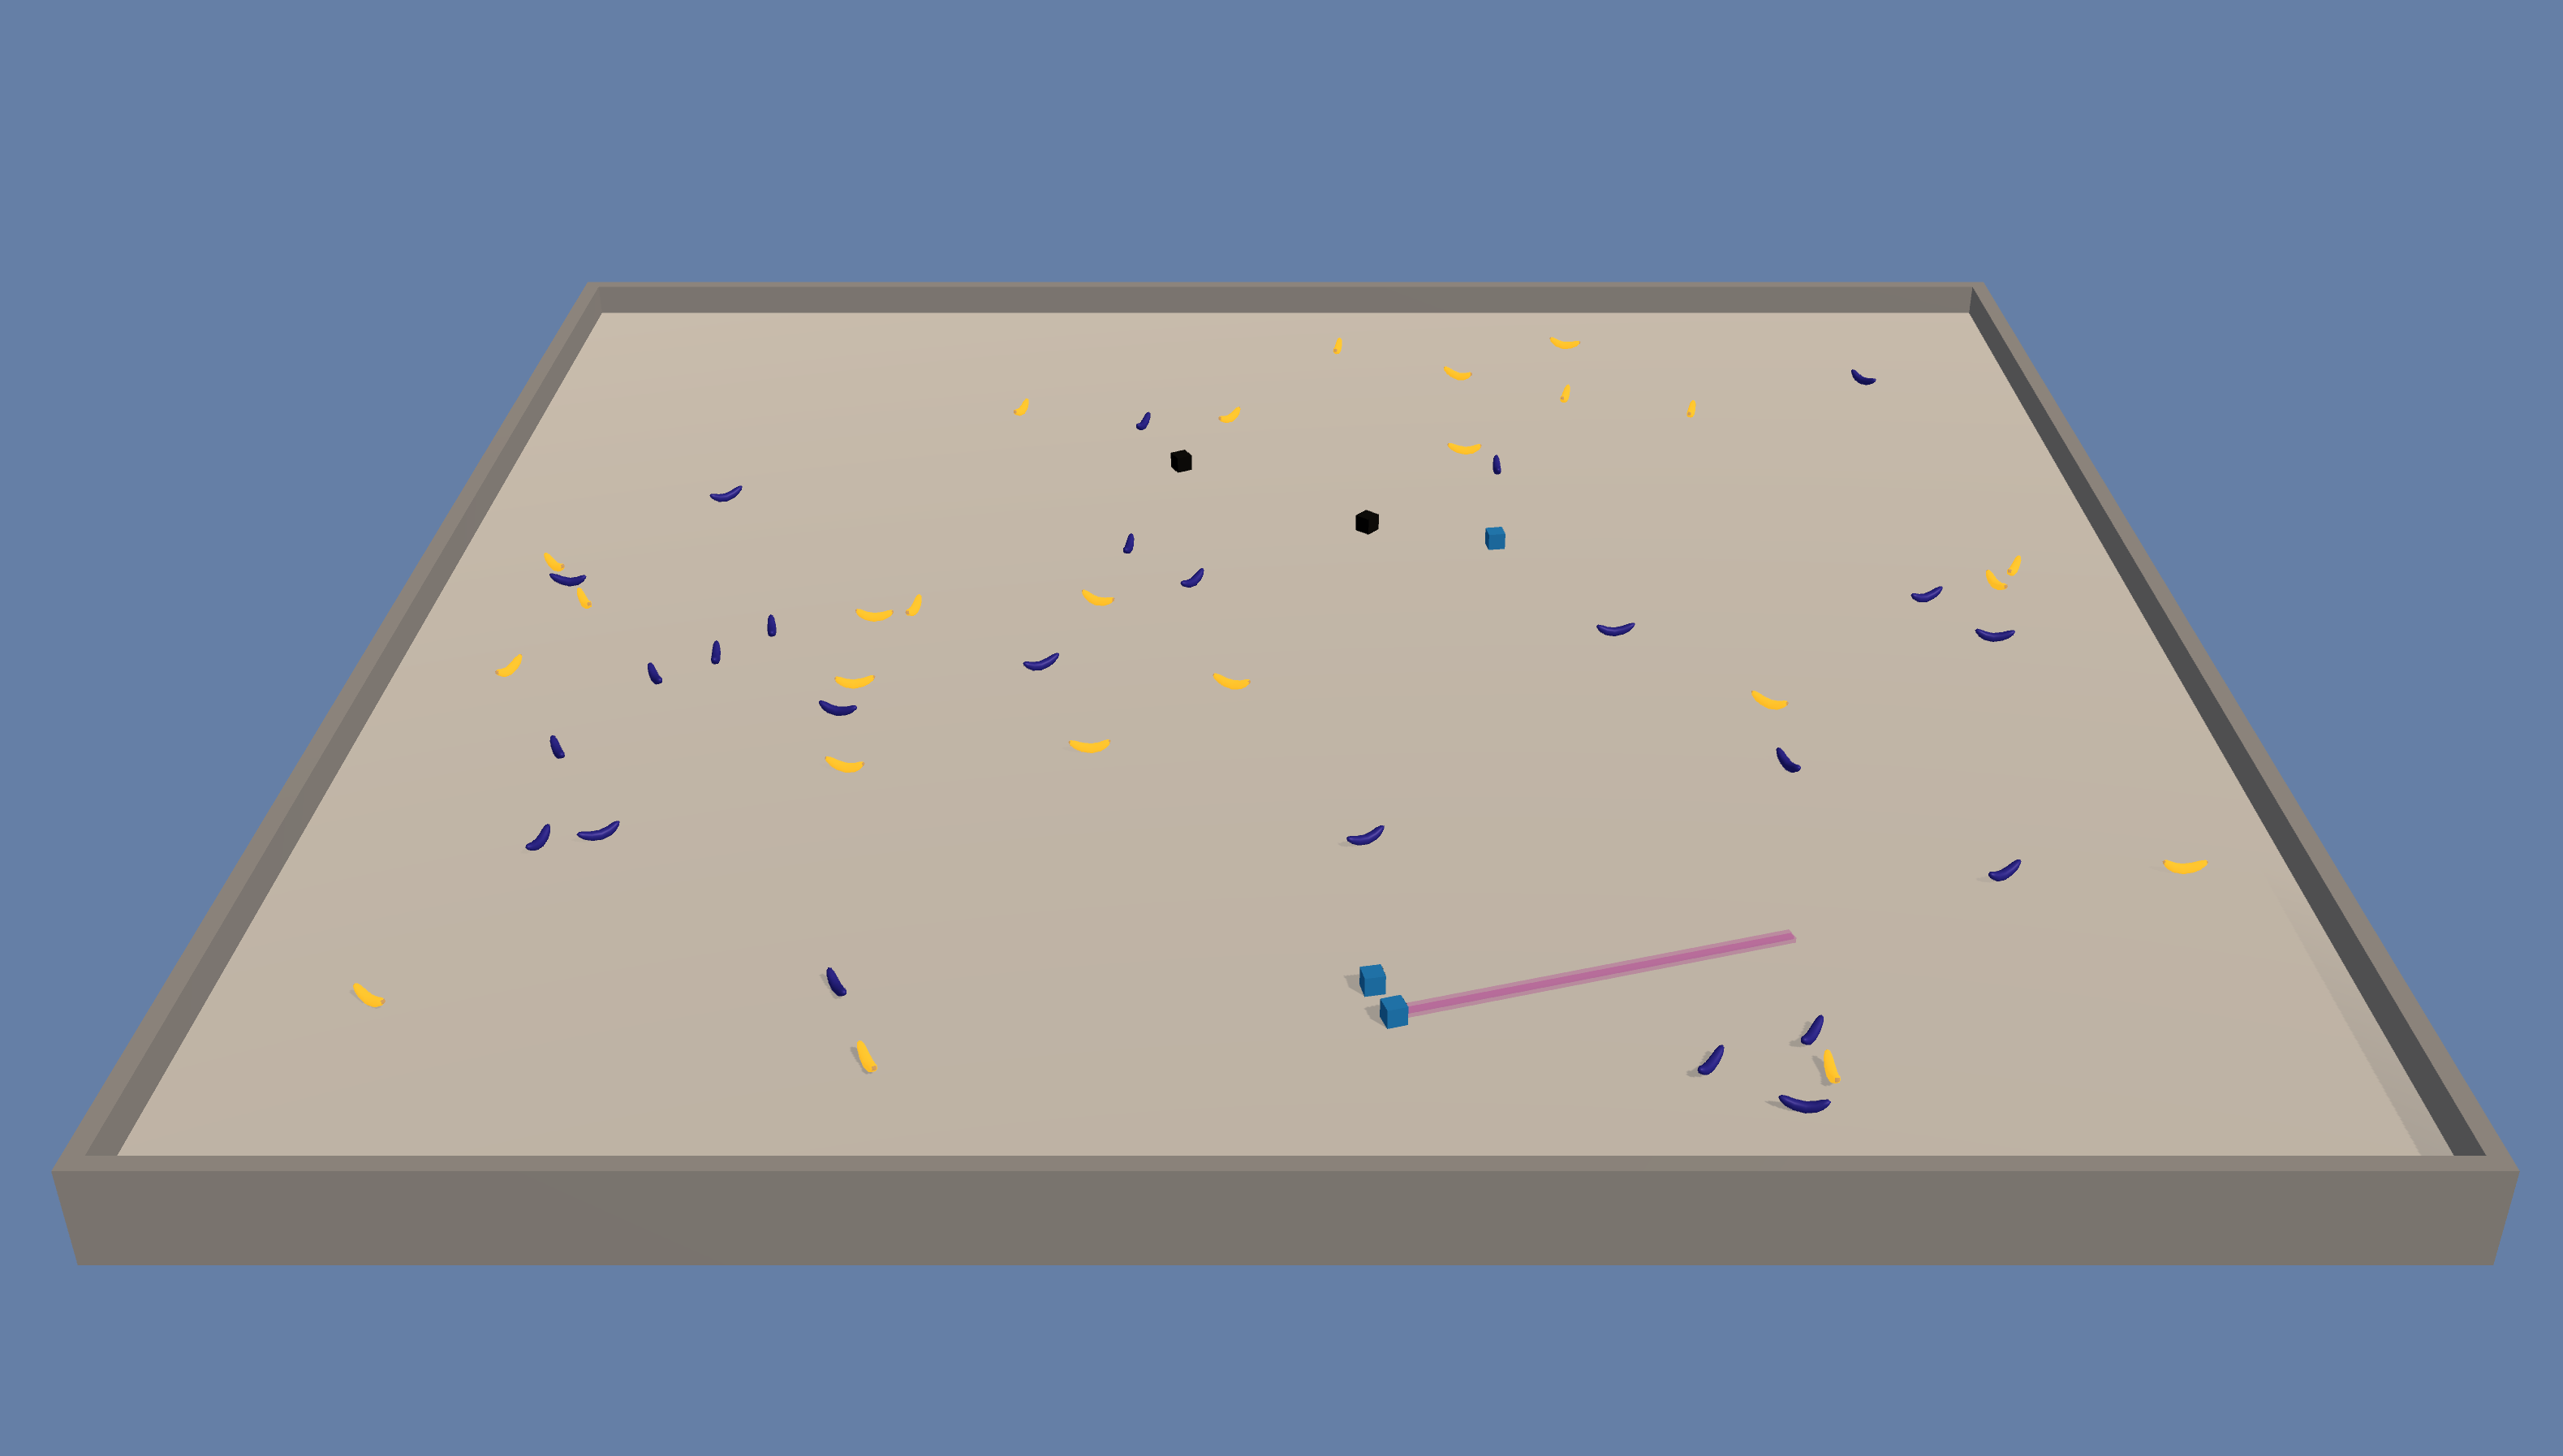
\includegraphics[height=1.5in]{images/banana.png}
   \caption{Unity ML-Agent: Banana Collector}
 }

\maketitle


\keywordlist

%% Required for all content. 

%%%%%%%%%%%%%%%%%%%%%%%%%%%%%%%%%%%%%%%%%%%%%%%%%%%%%%%%%%%%%%
%% Introduction                                                                                                                             %%
%%%%%%%%%%%%%%%%%%%%%%%%%%%%%%%%%%%%%%%%%%%%%%%%%%%%%%%%%%%%%%
\section{Introduction}

In this project I'll implement some solutions to the Unity ML-Agent 
\href{http://github.com/Unity-Technologies/ml-agents/blob/master/docs/Learning-Environment-Examples.md#banana-collector}{\underline{Banana Collector}}
 environment. In this environment an agent observes a 37 dimensional vector containing the agent's velocity, along with ray-based perception of 
objects around the agent's forward direction and tries to learn how to best select one of the following actions:
\begin{enumerate}
	\item move forward,
	\item move backward,
	\item turn left, and
	\item turn right.
\end{enumerate}
A reward of +1 is provided for collecting a yellow banana, and a reward of -1 is provided for collecting a blue banana.
Thus, the goal of the agent is to collect as many yellow bananas as possible while avoiding blue bananas.


I'll give the following three solutions:
\begin{enumerate}
	\item {\em Deep Q-Learning}~\cite{DBLP:journals/nature/MnihKSRVBGRFOPB15},
	\item {\em Double Deep Q-Learning}~\cite{DBLP:journals/corr/HasseltGS15}, and
	\item {\em Dueling Deep Q-Learning}~\cite{DBLP:journals/corr/WangFL15}. 
\end{enumerate}
Source code in Python, using PyTorch, is available on 
\href{http://github.com}{\underline{github}} 
in the repo 
\href{http://github.com/bobflagg/Deep-Q-Learning-for-Navigation}{\underline{Deep-Q-Learning-for-Navigation}}.
%%%%%%%%%%%%%%%%%%%%%%%%%%%%%%%%%%%%%%%%%%%%%%%%%%%%%%%%%%%%%%
%% Background                                                                                                                             %%
%%%%%%%%%%%%%%%%%%%%%%%%%%%%%%%%%%%%%%%%%%%%%%%%%%%%%%%%%%%%%%
\section{Background}

The Unity ML-Agent Banana Collector is a {\em sequential decision making problem}, in which an agent interacts with an environment over discrete time
steps and tries to find a {\em policy} to maximize the expected {\em discounted return}:
$$G_t = \sum_{\tau=t}^{\infty}\gamma^{\tau-t}R_\tau,$$
where $\gamma\in[0,1]$  is a discount factor that trades-off the importance of immediate and future rewards.
See~\cite{DBLP:books/lib/SuttonB98} for a general discussion of this sort of problem. 

In this project I'll focus on a particular class of algorithms for 
solving sequential decision making problems called {\em Q-Learning}. The main idea behind Q-Learning is that if we had a function 
$$Q^*:{\cal S} \times {\cal A}:\to\mathbb{R},$$
where ${\cal S}$ is the set of states and ${\cal A}$ is the set of possible actions, that could tell us what our return would be, if we were to take an action in a given state, then we could easily construct a policy that maximizes our rewards:
$$\pi^*(s) = \operatorname{arg\,max}_{a} Q^*(s,a).$$
Unfortunately we don't know enough about the environment to compute $Q^*(s,a)$. One approach to overcome this problem is 
{\em Q-learning}~\cite{DBLP:books/lib/WatkinsC1989}, 
an early breakthrough in reinforcement learning.   Q-learning approximates the optimal action-value function with a learned action-value function $Q(s,a)$, which 
is initialized randomly and then updated incrementally according to the formula
%% $$Q(S_t,A_t) \leftarrow Q(S_t,A_t) + \alpha \cdot \big[R_{t+1}+\gamma \cdot \max_a Q(S_{t+1},a) - Q(S_t,A_t)\big]$$
%% or
$$Q(S_t,A_t) \leftarrow (1-\alpha)\cdot Q(S_t,A_t) + \alpha \cdot \big[R_{t+1}+\gamma \cdot \max_a Q(S_{t+1},a)\big].$$
In the standard Q-learning implementation Q-values are stored in a table.
One cell is required per combination of state and action. This implementation
is not amenable to continuous state problems like the Unity ML-Agent Banana Collector.
The simplest way to get around this is to apply discretization but that scales poorly. As the number of
state and action variables increase, the size of the table used to store Q-values
grows exponentially. The next section describes an alternative to discretized Q-learning, which scales well.

%%%%%%%%%%%%%%%%%%%%%%%%%%%%%%%%%%%%%%%%%%%%%%%%%%%%%%%%%%%%%%
%% Deep Q-Learning for Navigation                                                                                                %%
%%%%%%%%%%%%%%%%%%%%%%%%%%%%%%%%%%%%%%%%%%%%%%%%%%%%%%%%%%%%%%
\section{ Deep Q-Learning for Navigation}

\begin{figure}[h]
	\centering
	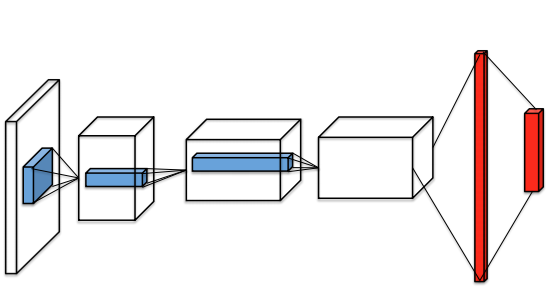
\includegraphics[width=3.0in]{images/dqn}
	\caption{Deep Q-Network~\protect\cite{DBLP:journals/corr/WangFL15}}
	\label{fig:dqn}
\end{figure}

Deep Q-learning is an alternative to discretized Q-learning, which addresses the scaling problem by approximating $Q^*(s,a)$ 
with a {\em deep Q-network}, $Q(s,a|\theta)$, and tuning the parameters by optimizing the following
of loss function:
$$L(\theta) = \mathbb{E}\big[\big(y^{DQN}-Q(S_t, A_t|\theta)\big)^2\big],$$
with 
$$ y^{DQN}=R_t+\gamma\cdot\max_{a'}Q(S_{t+1},a'|\theta^-),$$
where $\theta^-$ representes the parameters of a fixed and separate {\em target network}.

I've implemented deep Q-learning for the Unity ML-Agent Banana Collector in the notebook 
\href{https://nbviewer.jupyter.org/github/bobflagg/Deep-Q-Learning-for-Navigation/blob/master/01-Deep-Q-Learning-for-Navigation.ipynb}{\underline{Deep-Q-Learning-for-Navigation}}.
The Q-network has two fully connected linear layers each with 64 hidden units.   I trained for 500 episodes with a batch size of 64, discount factor of $\gamma = 0.99$, soft update weight of $\tau = 0.001$ and learning rate of $0.0005$.  The score plot is below and shows the evironment was solved in about 429 episodes.

\FloatBarrier
\begin{figure}[h]
	\centering
	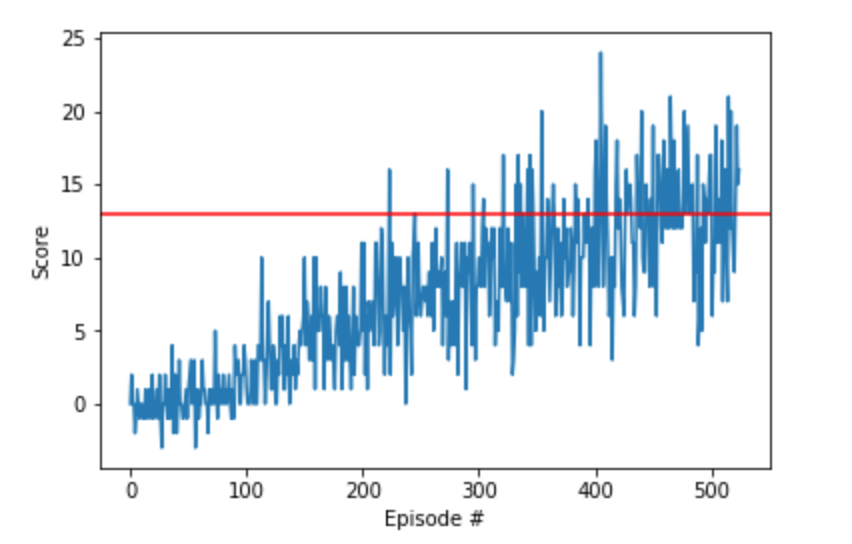
\includegraphics[width=3.0in]{images/dqn-scores}
	\caption{Scores for Deep Q-Learning}
	\label{fig:dqn-scores}
\end{figure}
\FloatBarrier

%%%%%%%%%%%%%%%%%%%%%%%%%%%%%%%%%%%%%%%%%%%%%%%%%%%%%%%%%%%%%%
%% Deep Q-Learning for Navigation                                                                                                %%
%%%%%%%%%%%%%%%%%%%%%%%%%%%%%%%%%%%%%%%%%%%%%%%%%%%%%%%%%%%%%%
\section{ Double Deep Q-Learning for Navigation}

In Q-learning and deep Q-learning, the max operator in the loss function uses the same values to both select and evaluate an action. 
This can lead to over optimistic value estimates.  {\em Double deep Q-learning} mitigates this problem by using a different target:
$$ y^{DDQN}=R_t+\gamma\cdot Q(S_{t+1},  \operatorname{arg\,max}_{a'} Q(S_{t+1}, a'|\theta)|\theta^-).$$

I've implemented double Q-learning for the Unity ML-Agent Banana Collector in the notebook 
\href{https://nbviewer.jupyter.org/github/bobflagg/Deep-Q-Learning-for-Navigation/blob/master/02-Double-Deep-Q-Learning-for-Navigation.ipynb}{\underline{Double-Deep-Q-Learning-for-Navigation}}.
I used a Q-network with two fully connected linear layers each with 64 hidden units.   I trained for 500 episodes with a batch size of 64, discount factor of $\gamma = 0.99$, soft update weight of $\tau = 0.001$ and learning rate of $0.0005$.  The score plot is below and shows the evironment was solved in about 427 episodes.

\begin{figure}[h]
	\centering
	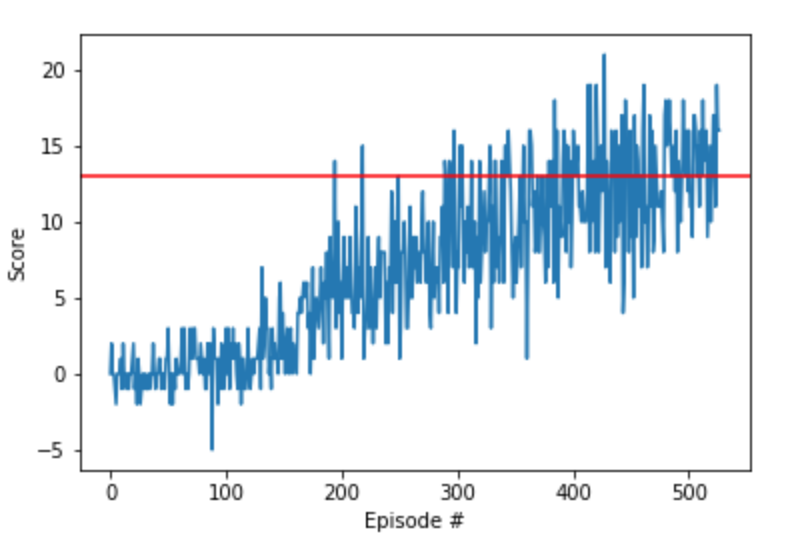
\includegraphics[width=3.0in]{images/double-dqn-scores}
	\caption{Scores for Double Deep Q-Learning}
	\label{fig:ferrari}
\end{figure}

%%%%%%%%%%%%%%%%%%%%%%%%%%%%%%%%%%%%%%%%%%%%%%%%%%%%%%%%%%%%%%
%% Deep Q-Learning for Navigation                                                                                                %%
%%%%%%%%%%%%%%%%%%%%%%%%%%%%%%%%%%%%%%%%%%%%%%%%%%%%%%%%%%%%%%
\section{ Dueling Deep Q-Learning for Navigation}

\begin{figure}[h]
	\centering
	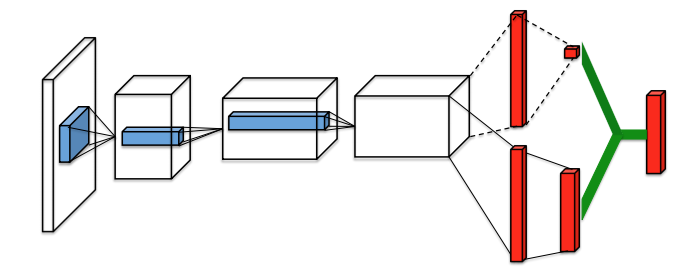
\includegraphics[width=3.0in]{images/dueling-dqn}
	\caption{Dueling Deep Q-Network~\protect\cite{DBLP:journals/corr/WangFL15}}
	\label{fig:dueling-dq}
\end{figure}

The architecture of the Q-network in dueling deep Q-learning has two streams, one, with paraameters $\theta, \alpha$, estimates the state-value function:
$$V(s) = \mathbb{E}\big[Q(s,A_t)\big]$$
and the other, with paraameters $\theta, \beta$,  estimates the expression 
$$A(s,a) - \frac{1}{{\cal |A|}}\sum_{a'}A(s, a'),$$
where 
$$A(s,a) = Q(s,a) - V(s).$$
is the {\em advantage function}, which provides a relative measure of the importance of each action for a given state.

The estimate of the action-value function is then
$$Q(s,a|\theta, \alpha, \beta) = V(s|\theta, \beta) - \big(A(s,a|\theta, \alpha) - \frac{1}{{\cal |A|}}\sum_{a'}A(s, a'|\theta, \alpha)\big).$$
As Figure ~\ref{fig:dueling-dq} illustrates, the two streams share some weights, $\theta$, but have separate heads with independent parameters, $\alpha$ and $\beta$.  I don't use convolution in the network for the Unity ML-Agent Banana Collector so the shared $\theta$ parameters in this example are for a couple of simple fully connected layers.

Since the output of the dueling network is a $Q$ function, it can be trained with the many existing algorithms. I tried Deep Q-Learning and Double Deep Q-Learning. 
In both experiments I used a Dueling Q-Network with a shared fully connected linear layer with 64 hidden units, a fully connected linear layer with 64 hidden units for
the advantage head and a fully connected linear layer with 64 hidden units for the value head.  I trained for 500 episodes with a batch size of 64, discount factor of $\gamma = 0.99$, soft update weight of $\tau = 0.001$ and learning rate of $0.0005$.  The score plots are below.  Dueling Deep Q-Learning solved the environment in after 339 episodes.

\begin{figure}[h]
	\centering
	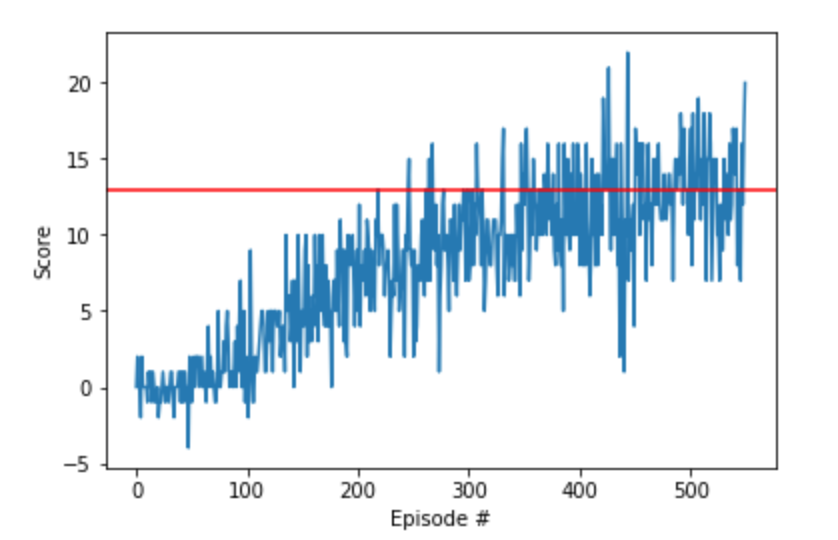
\includegraphics[width=3.0in]{images/dueling-dqn-scores}
	\caption{Scores for Dueling Deep Q-Learning}
	\label{fig:dueling-dqn-scores}
\end{figure}



\begin{figure}[h]
	\centering
	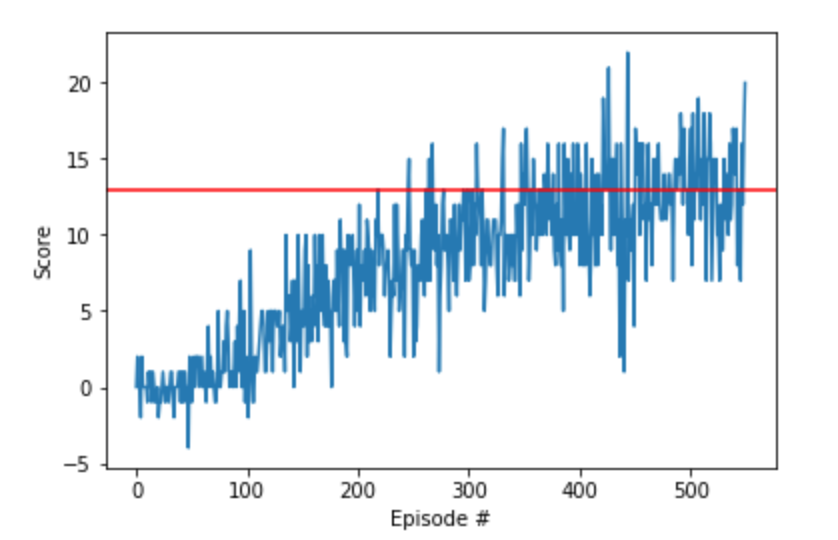
\includegraphics[width=3.0in]{images/dueling-double-dqn-scores}
	\caption{Scores for Dueling Double Deep Q-Learning}
	\label{fig:dueling-double-dqn-scores}
\end{figure}


%%%%%%%%%%%%%%%%%%%%%%%%%%%%%%%%%%%%%%%%%%%%%%%%%%%%%%%%%%%%%%
%% Deep Q-Learning for Navigation                                                                                                %%
%%%%%%%%%%%%%%%%%%%%%%%%%%%%%%%%%%%%%%%%%%%%%%%%%%%%%%%%%%%%%%
\section{Improving Performance}

Dueling Deep Q-Learning performed best in the experiments I did.  To improve performance futher, I would do grid search on the hyper-parameters and network architecture for this approach.  Another interesting direction would be {\em prioritized replay}~\cite{DBLP:journals/corr/SchaulQAS15}, which is
 built on top of DDQN.  Their key idea is
to increase the replay probability of experience tuples
that have a high expected learning progress (as measured
via the proxy of absolute TD-error). This has led to both
faster learning and to better final policy quality across
many environments.

\bibliographystyle{acmsiggraph}
%\bibliographystyle{abbrv}
%%\nocite{*}
\bibliography{main}
\end{document}